\section{Общая часть}
    \subsection{Частотно-регулируемый электропривод}
        В общем случае под электроприводом понимают электромеханическую
        систему, приводящую в движение рабочие органы технического устройства и
        состоящую из передаточного, электродвигательного, преобразовательного и
        управляющего устройств. Электропривод, который в качестве
        преобразовательного устройства использует преобразователь частоты,
        называется частотно-регулируемый привод (ЧРП). 

        Принцип частотного регулирования, при котором частота и напряжение
        питания двигателя могут изменяться в соответствии с установленным
        соотношением независимо друг от друга, является наиболее эффективным
        способом управления скоростью асинхронных двигателей. Реализация такого
        способа определяется тем, что скорость вращающегося магнитного поля
        статора $\omega_0$  пропорциональна частоте источника питания $f$
        \begin{equation}
            \label{eq:w0}
            \omega_0 = \frac{2\pi f}{p},
        \end{equation}

        где $p$ -- число пар полюсов электродвигателя;

        $f$ -- частота напряжения переменного тока питающей сети двигателя.
        
        Следовательно, изменяя частоту $f$,
        можно плавно и в широких пределах регулировать скорость вращения
        ротора. 

        Скольжение определяется по формуле
        \begin{equation}
            \label{eq:slip}
            S = \frac{\omega_0 - \omega_\text{н}}{\omega_0}.
        \end{equation}
        
        При этом скольжение изменяется незначительно и, следовательно, потери,
        пропорциональные величине скольжения, также изменяются незначительно.
        Это важное преимущество частотного управления асинхронным двигателем
        позволяет реализовать энергосберегающие технологии как для двигателей с
        фазным ротором, так и с короткозамкнутым.

        Из изложенного вытекает, что для частотно-регулируемого асинхронного
        привода требуется прежде всего источник переменного тока регулируемой
        частоты. Использование для этих целей синхронных генераторов с
        регулируемой скоростью вращения не оправдывается ни техническими, ни
        экономическими соображениями. Только при появлении статических
        полупроводниковых преобразователей возникла реальная возможность
        создания частотно-регулируемых промышленных электроприводов. Их основу
        составляют преобразователь частоты и асинхронный двигатель (ПЧ-АД).
        
        Основной выходной координатой силового привода является
        электромагнитный момент. При частотном управлении его значение зависит
        от частоты и напряжения источника переменного тока
        \begin{equation}
            \label{eq:Md}
            M_\text{д} = \frac{m_c U^2 r_c}{\omega_0 S \left[ (r_c+r_p S^{-1})^2+
                (X_c+X_p)^2\right]},
        \end{equation}

        где $m_c$ -- число фаз;

        $U$ -- напряжение, подводимое к статору двигателя;

        $r_c, r_p, X_c, X_p$ -- активные и индуктивные сопротивления статорной
        и роторной цепей.

        Поэтому наличие двух независимых каналов управления дает возможность
        реализовать в системах ПЧ-АД различные законы регулирования с скорости.
        Если должна сохраняться постоянной перегрузочная способность двигателя,
        то в первом приближении частотный закон управления имеет вид
        \begin{equation}
            \label{eq:UUs}
            \frac{U}{U_c} = \frac{f}{f_c} \cdot \sqrt{\frac{M}{M_\text{н}}},
        \end{equation}

        где $U_c, f_c$ -- номинальные напряжение и частота сети;

        $U, f$ -- напряжение и частота на выходе ПЧ;

        $M_\text{н}, M$ -- номинальное и текущее значение момента АД.

        Управление двигателем в соответствии с соотношением (\ref{eq:UUs}) при
        ненасыщенной магнитной системе позволяет сохранять практически
        неизменным коэффициент мощности и абсолютное скольжение электропривода,
        при этом его КПД не зависит от скорости. В этом и заключается основное
        достоинство частотного управления.

        В зависимости от видов нагрузки закон управления напряжением и частотой
        имеет различные формы. Например, при постоянном моменте нагрузки
        ($M_c=const$) соотношение (\ref{eq:UUs}) приобретает вид $U/f=const$.
        Механические характеристики привода ПЧ-АД, сохраняющего постоянство
        перегрузочной способности двигателя, приведены
        на рисунке \ref{fig:mech}.
        \vspace{1cm}

        \begin{figure}[h!]
            \center{
                %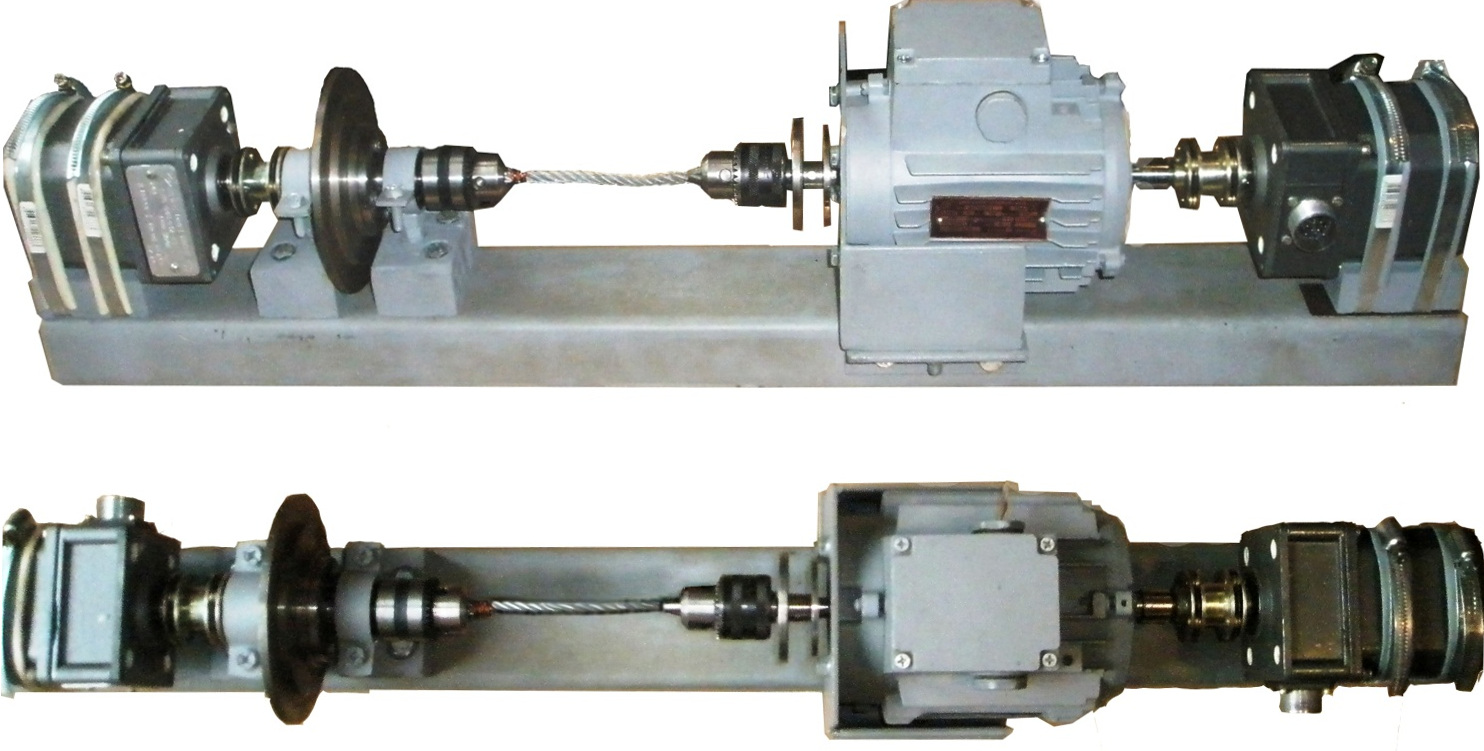
\includegraphics[width=0.8\linewidth]{img/general-view}
                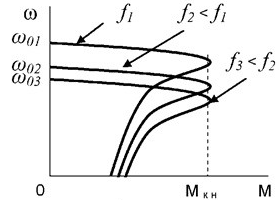
\includegraphics{img/mech}
            }
            \caption{Механическая характеристика привода ПЧ-АД}
            \label{fig:mech}
        \end{figure}

        Таким образом, для того, чтобы реализовать принцип частотного
        управления асинхронным двигателем, необходимо в соответствии с
        выражением (\ref{eq:UUs}) и с учетом вида нагрузки управлять напряжением,
        подводимым к статору двигателя, взаимосвязано с изменением частоты
        питания.

        Функцию преобразования параметров электрической энергии питающей сети к
        таким значениям, которые необходимы для нормальной работы приводного
        двигателя, а также функцию дозирования величины электрической энергии,
        подводимой к двигателю для регулирования его скорости и выполняет
        преобразовательное устройство.

        В системах регулируемого электропривода находят применение все основные
        типы преобразовательных устройств: выпрямители, преобразующие
        переменное напряжение в постоянное, инверторы, осуществляющие обратное
        выпрямителям преобразование энергии, непосредственные преобразователи
        частоты, регуляторы переменного и постоянного напряжения,
        обеспечивающие преобразование уровня напряжения без изменения его
        частоты.

        Эффективность применения и перспективы дальнейшего использования тех
        или иных преобразовательных устройств в значительной степени
        определяется совершенством свойств силовых полупроводниковых приборов.

        Следует учитывать главную особенность силовых преобразователей
        электрической энергии независимо от типа и свойств, применяемых
        силовых полупроводниковых приборов они должны использоваться только в
        ключевых режимах работы, для которых свойственны два устойчивых
        состояния полного включения (максимальная электрическая проводимость) и
        полного выключения (минимальная проводимость). Исключением являются
        только динамические процессы, связанные с переходами из одного
        устойчивого состояния в другое. В состояниях ключевого режима потери
        активной мощности $P=UI$ в полупроводниковых приборах малы, поскольку
        один из сомножителей этого произведения (ток I или напряжение U) ,
        имеет минимально возможное значение. Это и обеспечивает высокий КПД
        полупроводниковых преобразователей электрической энергии.

        Наиболее распространенным типом преобразователей частоты является
        двухступенчатое преобразовательное устройство, выполненное на основе
        выпрямителя трехфазного переменного напряжения сети и автономного
        инвертора напряжения (АИН), преобразующего выпрямленное напряжение в
        переменное трехфазное с регулируемой частотой и амплитудой. Несмотря на
        двухкратность преобразования энергии и обусловленное этим некоторое
        снижение КПД, такие преобразователи частоты (с промежуточным звеном
        постоянного тока) получили наибольшее распространение в различных типах
        электроустановок. В отличие от АИТ, содержащего на своем входе в цепи
        постоянного тока индуктивность, обязательным элементом на входе АИН
        является параллельно включенная емкость. Поэтому в результате
        подключений полупроводниковыми ключами этой емкости к выходным зажимам
        АИН осуществляется формирование кривых напряжения нагрузки. При
        использовании неуправляемого выпрямителя обеспечивается высокое
        значение коэффициента мощности на входе, а регулирование величины
        выходного напряжения может осуществляться методом широтноимпульсной
        модуляции (ШИМ).

        Метод двуполярной ШИМ является частным случаем ШИР, при котором
        соотношение ширины импульсов противоположной полярности на протяжении
        каждой полуволны выходного напряжения изменяется таким образом, чтобы
        среднее значение каждой пары импульсов за период их частоты следования
        (частоты ШИМ) равнялось мгновенному значению основной гармоники
        выходного напряжения в середине интервала усреднения. Кривая выходного
        напряжения (однофазного) АИН для такой двуполярной ШИМ показана на
        рисунке \ref{fig:pwm}.

        \begin{figure}[h!]
            \center{
                %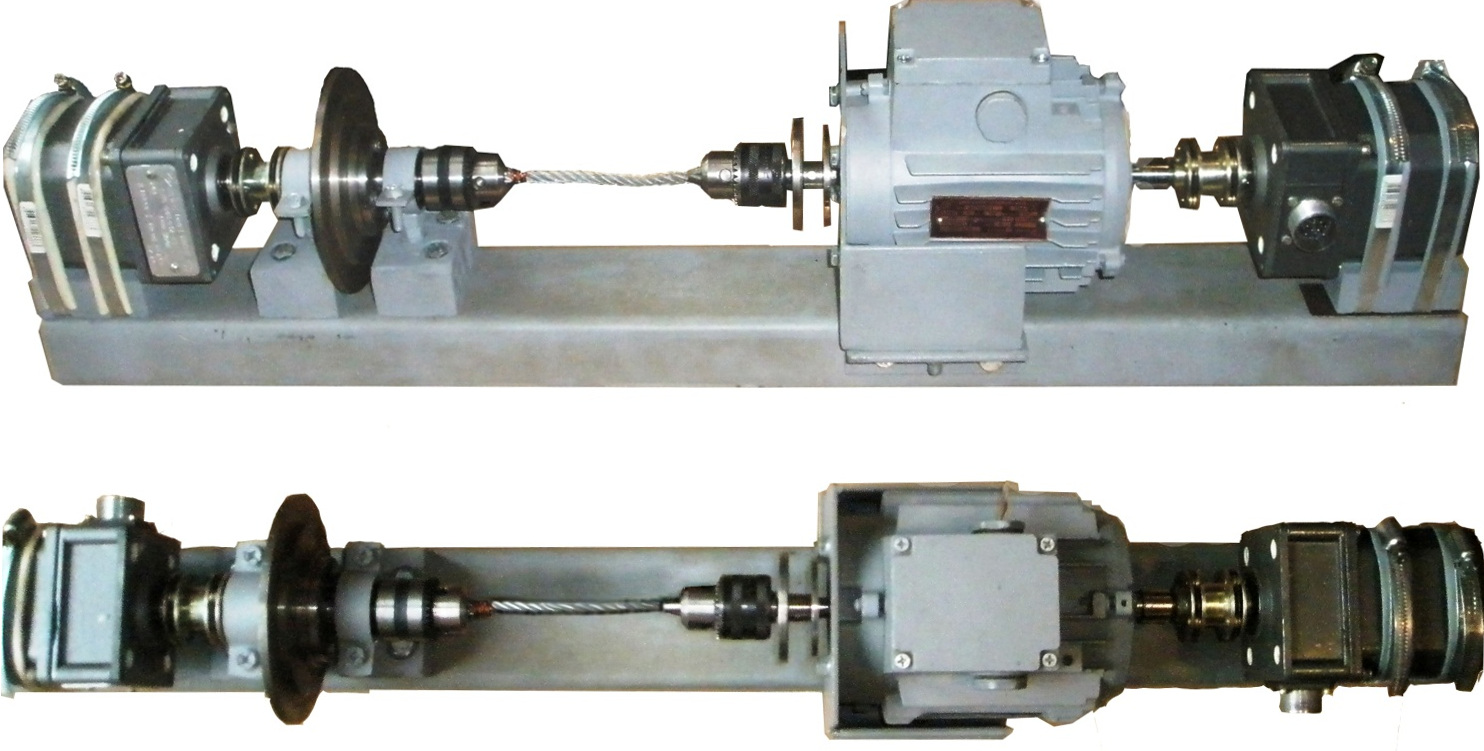
\includegraphics[width=0.8\linewidth]{img/general-view}
                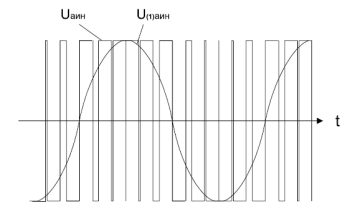
\includegraphics{img/pwm}
            }
            \caption{Форма выходного напряжения однофазного АИН с ШИМ
                $U_\text{(1)аин}$ - основная гармоника}
            \label{fig:pwm}
        \end{figure}
        
        При формировании выходных напряжений трехфазного АИН каждая из фаз
        нагрузки в любой момент времени оказывается подключенной к одному из
        двух полюсов входного постоянного напряжения. Поэтому в момент
        подключения данной фазы к одному полюсу возможны три комбинации
        подключений двух других фаз
        \begin{itemize}
            \item обе фазы подключены к тому же полюсу;
            \item одна из фаз подключена к тому же полюсу, а другая к противоположному;
            \item обе фазы подключены к противоположному полюсу напряжения. 
        \end{itemize}

        Следовательно, мгновенное напряжение каждой фазы трехфазного АИН может
        принимать значения, соответствующие пяти уровням. Пример кривой
        выходного напряжения трехфазного АИН с ШИМ показан на рисунке
        \ref{fig:3ph-pwm}. Частота высших гармонических составляющих выходного
        напряжения определяется частотой ШИМ, которая при использовании в АИН
        современных транзисторов типа IGBT может без заметного снижения КПД
        преобразователя повышена до величины более 4 кГц. Поэтому, несмотря на
        значительный уровень амплитуды высших гармоник напряжения АИН, токи ак
        тивно-индуктивной нагрузки (например, асинхронный двигатель)
        практически синусоидальны.

        \begin{figure}[h!]
            \center{
                %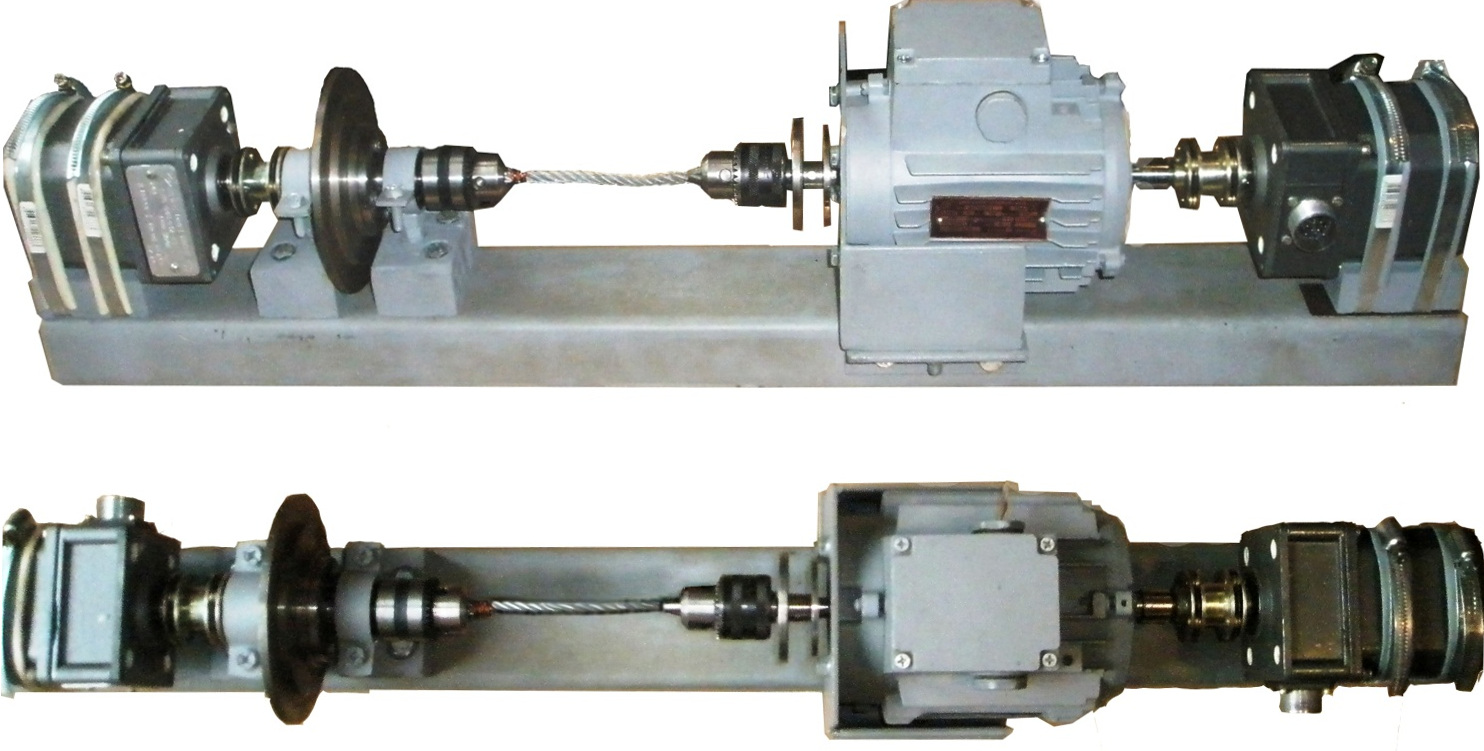
\includegraphics[width=0.8\linewidth]{img/general-view}
                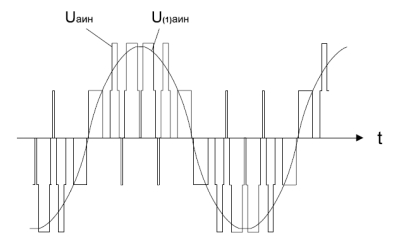
\includegraphics{img/3ph-pwm}
            }
            \caption{Форма выходного напряжения одной фазы трехфазного АИН с ШИМ}
            \label{fig:3ph-pwm}
        \end{figure}

        Кратко остановимся на тормозных режимах частотно-регулируемого
        электропривода. Этот режим может быть осуществлен по принципу
        динамического торможения при питании обмоток статора двигателя
        постоянным током от АИН. В случаях, когда эффективность такого
        торможения оказывается недостаточной, может быть использован принцип
        генераторного торможения с передачей активной мощности через АИН в цепь
        постоянного тока преобразователя частоты. Поскольку передача энергии в
        сеть через неуправляемый выпрямитель невозможна, для предотвращения
        недопустимого повышения напряжения на емкости фильтра постоянного тока
        ее разряжают с помощью транзисторного импульсного регулятора на
        специальный тормозной резистор. 

        Таким образом, анализ состояния вопроса показал, что оптимальную по
        энергетическим показателям и по регулировочным и механическим
        характеристикам структуру современного частотно-регулируемого
        асинхронного электропривода следует выполнять на основе преобразователя
        частоты с промежуточным звеном постоянного тока (рисунок
        \ref{fig:ain}).

        \begin{figure}[h!]
            \center{
                %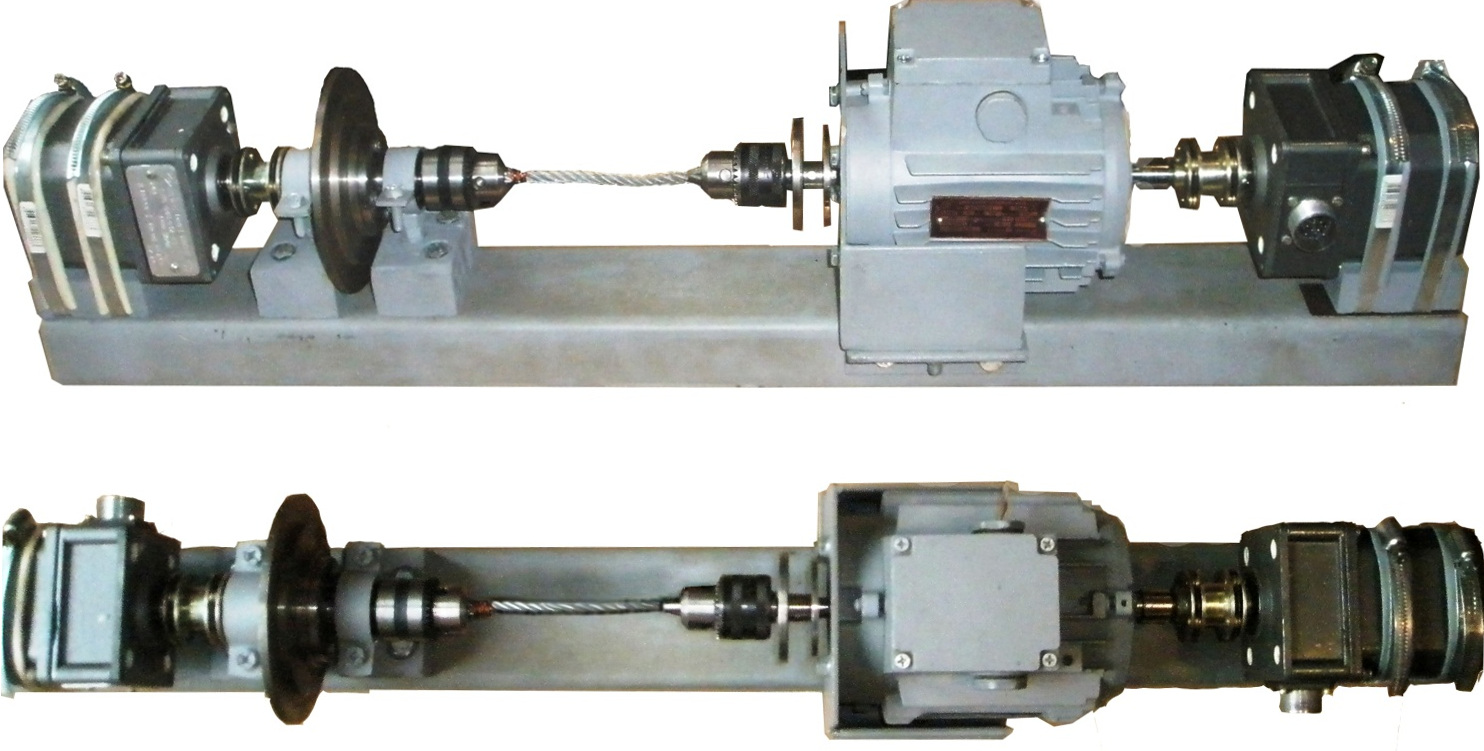
\includegraphics[width=0.8\linewidth]{img/general-view}
                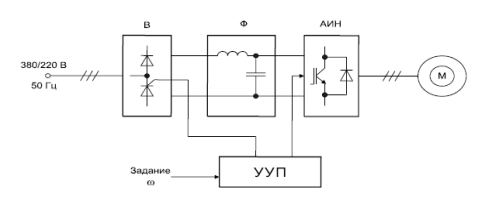
\includegraphics{img/ain}
            }
            \caption{Частотно регулируемый электропривод.}
            \label{fig:ain}
        \end{figure}
        
        Частотно регулируемый электропривод состоит из выпрямителя с
        индуктивно-емкостным фильтром постоянного напряжения и автономного
        инвертора напряжения, построенного на силовых транзисторах типа IGBT и
        формирующего основную гармонику выходного напряжения методом
        широтно-импульсной модуляции.  Регулируемый электропривод, силовая
        часть которого базируется на структуре, представленной на рисунке
        \ref{fig:ain}, обладает целым рядом достоинств -- широким диапазоном
        регулирования (D=30-100 и более), высоким коэффициентом полезного
        действия (без учета двигателя он достигает величины 0,98), высоким
        коэффициентом мощности (до 0,98), высокой надежностью и компактностью
        преобразователя и др. 

        \clearpage

